\documentclass[ngerman]{handout}
\usepackage[
  type={CC},
  modifier={by-sa},
  version={4.0},
  imagemodifier={-eu-80x15},
]{doclicense}

\usepackage[backend=biber, style=numeric, sorting=none]{biblatex}
\addbibresource{ref.bib}
\renewcommand*{\bibfont}{\scriptsize}

\date{2023-03-07}
\author{C. Badermann}
\title{Handout -- Die Speicherkarte}
\location{Gelsenkirchen}

\begin{document}
  \maketitle\\

  \begin{multicols*}{2}
    \handsec{Qualitäten von SD-Karten}
    Für integrierte Systeme wie die Arduino Plattform ist die microSD-Karte ein geeignetes Medium für die nichtflüchtige Speicherung von Daten.
    Diese sind \href{https://de.wikipedia.org/wiki/Flash-Speicher}{Flash-EEPROM} nach Standard der \enquote{SD Association}.\\
    Sie erlauben die nichtflüchtige (bestehende) und alleinstehende Speicherung (ohne externe Systeme).\\

    Sie sind durch ihre Allgegenwärtigkeit und folgende Qualitäten präferiert:
    microSD-Karten besitzen ein beachtliches Volumen zu Speichervolumen Verhältnis, und sind kostengünstig. Ihre Verwendung ist mühelos, Anschlüsse sind häufig verfügbar, und sie verfügen über eine simple SPI-Schittstelle.\\

    \handsec{Hardware}
    \handsubsec{SD-Karte}
    Die Hardware von (micro-) SD Karten ist durch einen Standard der \enquote{SD Association} festgelegt.
    Dieser Spezifiziert z.B.: Funktionsweise \& Dimensionen der Produkte, welche unter dem \emph{SD} Warenzeichen verkauft werden dürfen.\\

    In miroSD-Karten sind Maße von etwa 11x15x1{mm}, sowie eine wohl definierte Schnittstelle zu erwarten.
    Eine Kerbe ermöglicht das Einrasten in Lesegeräte.

    Im inneren der Karten sind unter anderem der Flash-Speicher, sowie ein Mikrocontroller zu finden.
    Letzterer stellt nutzerfreundliche Protokolle zur strukturierten Nutzung des Speichers zur Verfügung.

    \handsubsec{Interfaces}
    Zur Verbindung des Arduino mit SD-Karten gibt es verschiedene Schnittstellen.
    Häufig sind Shields mit microSD Anschluss und Breakout-Boards,
    welche die Kontakte der SD-Karte zur Verfügung stellen und ggf. die Stromstärke regulieren.
    Durch beide wird die Karte an den SPI-Bus des Arduino angehangen.

    \handsec{Formatierung}
    Zur Verwendung von microSD-Karten mit dem Arduino, müssen diese gegebenenfalls formatiert werden.
    Unterstützt werden MBR / DOS oder die kompatible GUID-Partitionstabellen mit den FAT-16 / 32 Dateisystemen\cite{sd-lib}.\\

    Nicht integrierte System nutzen häufig SD-Bus, UHS-II Bus, oder PCIe, anstelle von SPI.
    Dies erlaubt für Karten mit größeren Speichervolumen und höheren Transfergeschwindigkeiten.
    Für den Arduino ist dies insofern relevant, als diese nicht direkt verfügbar sind.
    Bestimmte Konfigurationen des SD Standards können nicht verwendet werden\cite{sd-spec_physical-layer}.

    \handsec{Die SD-Library}
    Die SD-Library bietet eine simple Abstraktionsebene über an den SPI-Bus angehangene SD-Karten.
    Sie kann durch den Library-Manager installiert, und als \enquote{\texttt{SD.h}} eingebunden werden.
    Zur Kommunikation über den SPI-Bus wird ebenfalls \enquote{\texttt{SPI.h}} benötigt.\\

    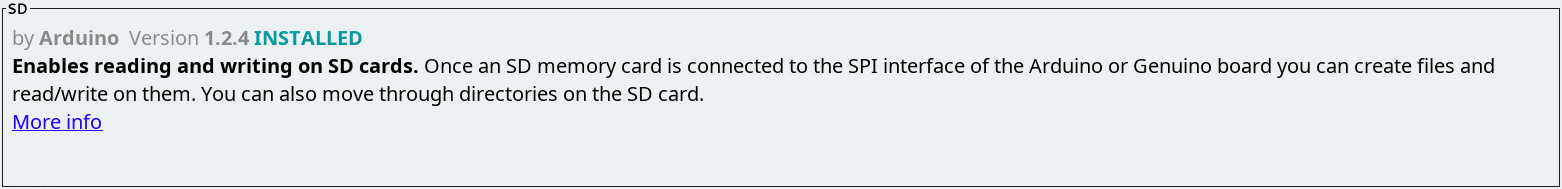
\includegraphics[width=\linewidth]{media/sd-lib.png}~\\

    Um die Verbindung herzustellen, wird die Funktion \enquote{\texttt{SD.begin(int cs)}} verwendet.
    Ihr Argument, \texttt{cs}, ist der \enquote{\texttt{Chip-Select Pin}} der SPI-Verbindung.
    Es liefert einen Boolean (Wahr / 1 bei Erfolg, Falsch / 0 bei Versagen).
    Dies kann mit einer If-Abfrage abgefangen werden, um den Programmfluss zu ändern, und ggf. Nutzer zu informieren.\\

    \handsubsec{Bearbeitung von Dateien}
    Dateien sind die idiomatischen Container für Daten.\\
    Um sie zum Lesen und oder Schreiben zu öffnen, wird \enquote{\texttt{SD.open(dateipfad, modus)}} verwendet.
    Dies liefert das \texttt{File} Objekt, welches für weitere Operationen auf die Datei benötigt wird.\\

    Modi beschreiben welche Aktionen auf die Datei ausgeführt werden können, z.B.: \texttt{File\_READ}
    \& \texttt{FILE\_WRITE}. Diese setzen sich ggf. aus weiteren Attributen zusammen. \texttt{File\_WRITE} = (\texttt{O\_READ} | \texttt{O\_WRITE} | \texttt{O\_CREAT} | \texttt{O\_APPEND}).
    Es erlaubt demnach das Lesen, Schreiben, sowie Erstellen von Dateien, falls diese nicht bereits existieren.
    Es schreibt ans Dateiende. Sie können auch eigens gesetzt werden.

    \tsec{Attribute bestehen wiederum aus simplen Ganzzahlen:
    \hspace*{1em}\texttt{uint8\_t const O\_READ = 0X01;}\\
    \hspace*{1em}\texttt{uint8\_t const O\_APPEND = 0X04;}.\\
    Bemerke; die Werte wurden als Zweierpotenzen ($2^n$) gewählt. Dies hat den Effekt, dass sie sich durch die \href{https://de.wikipedia.org/wiki/Disjunktion}{binäre Disjunktion} \enquote{\texttt{|}} kombinieren lassen:\\
    \hspace*{1em}\texttt{O\_READ | O\_APPEND = 0b001 | 0b100 = 0b101)}\\
    (mehr dazu in \href{https://github.com/arduino-libraries/SD}{\texttt{SD.h} \& \texttt{SDFat.h}})}\\

    Um Inhalte in Dateien zu schreiben, werden die bekannten \texttt{print()} Befehle auf das File Objekt angewandt.
    \texttt{write()} kann verwendet werden, um Binärdaten zu schreiben.
    \texttt{read()} ermöglicht das Lesen aus Dateien, so weit wie durch \texttt{available()} angegeben, weitere Daten vorhanden sind.

    \handsubsec{Dateisystemmanagement}
    Die Bearbeitung des Dateisystems per \enquote{\texttt{SD.h}} ist durch die Funktionen \texttt{open()}, \texttt{mkdir()}, \texttt{rmdir()}, \texttt{remove()} möglich.
    Durch Abfragen wie \texttt{exists()}, \texttt{isDirectory()}, \texttt{name()}, können existierende Strukturen ertastet werden.
    Per \texttt{open()}, \texttt{openNextFile()}, \texttt{rewindDirectory()} ist das Dateisystem zu navigieren.
    Beide \enquote{\texttt{open}} Funktionen sind ebenfalls für Ordern geeignet.

    \handsubsec{Zu Beachten}
    Das \texttt{File} Objekt erbt von \texttt{Stream} (Wie auch \texttt{Serial}) und ist somit gepuffert.
    Änderungen werden nicht direkt, sondern erst bei \texttt{flush} Ereignissen geschrieben.
    Dies geschieht z.B.: durch die \texttt{flush()} Funktion oder das Schließen einer Datei.
    Wird nicht geflushed, können Änderungen verloren gehen.\\

    Versionsbedingt ist ggf. nur eine Datei an einem Zeitpunkt zu öffnen.
    Auch das mehrfache Öffnen derselben Datei ist davon betroffen.
    Das Schließen von Dateien sollte somit nicht vergessen werden.\\

    Unterstützt sind lediglich \href{https://de.wikipedia.org/wiki/8.3}{8.3 Dateinamen} in Großbuchstaben\cite{sd-lib}.\\

    \tsec{Gegensätzlich zum \enquote{c} \texttt{FILE}, wird das \texttt{File} Objekt der SD Library bis auf den ersten Buchstaben kleingeschrieben.}

    \handsec{Speicherformate}
    Die Strukturierung der gesammelten Daten ist ein wichtiger Aspekt und bedeutend für die spätere Verarbeitung.
    Nutzerfreundlich sind textbasierte Formate; diese sind völlig plattformunabhängig und können ohne weiteres Eingelesen werden.
    Um die Weiterverarbeitung zu erleichtern, wird häufig strukturierter Text verwendet.
    Tabellen-artige Strukturen sind gut in CSV darzustellen.
    Datenserialisierungssprachen eignen sich für komplexere Strukturen, welche Computerlesbar gespeichert werden
    sollen. Hier findet sich z.B.: XML, YAML, JSON.\\

    \href{https://de.wikipedia.org/wiki/Bin\%C3\%A4rdatei}{Binärformate} können wesentlich platzsparender,
    und dadurch, aber auch durch die nicht notwendigen Umwandlungsprozesse weniger zeitraubend sein.
    Das Einlesen dieser auf anderen Systemen ist jedoch deutlich komplizierter.
    Existierende Formate wie Protobuf, oder BSON können dies erleichtern.
    Individuelle Formate sind anspruchsvoller, aber nicht selten und bieten mehr Flexibilität.\\

    Zu erwarten, sind ebenfalls menschliche oder technische Fehler.
    Von Daten, welche einen Wert haben, sollten stets unabhängige Sicherheitskopien existieren.
    Idealerweise auf mehreren Geräten oder sogar an mehreren Standorten\cite{chervenak-backup}.\\

    \handsubsec{CSV}
    Da eine Reihe durch Sensoren wiederholt gemessener Eigenschaften gut in einer Tabelle dargestellt werden kann, wurde für das Projekt \enquote{Wetterstation} das CSV / comma-separated values (RFC 4180) Format gewählt\cite{rfc4180}.\\

    Datenfelder / Spalten sind durch das Komma \enquote{\texttt{,}} getrennt.
    Zeilen durch die \href{https://de.wikipedia.org/wiki/Zeilenumbruch}{Zeilenumbruchsequenz}
    \enquote{\texttt{LF}} (\texttt{\textbackslash n}\footnote{\label{c-esc-seq}Dies sind die Zeichenfolgen, welche \texttt{c} für die genannten \href{https://de.wikipedia.org/wiki/Steuerzeichen}{ASCII Steuerzeichen} nutzt. Siehe: \href{https://de.wikipedia.org/wiki/Escape-Sequenz\#C}{https://de.wikipedia.org/wiki/Escape-Sequenz\#C}.})
    oder \enquote{\texttt{CR LF}} (\texttt{\textbackslash r \textbackslash n}\footnote{Siehe: \autoref{c-esc-seq}.}).
    Diese werden ebenfalls bei Betätigung von \keys{\return} in Texteingabefeldern eingefügt, sind aber häufig nicht explizit dargestellt.

    \lstinputlisting[caption={\footnotesize Beispiel CSV-Datei: (\href{https://de.wikipedia.org/w/index.php?title=CSV_(Dateiformat)\&oldid=229431469\#Beispiel}{Wikipedia -- CC BY-SA 3.0})}]{./media/sketch/csv.csv}

    \handsec{Beispielprojekt Wetterstation}
    Mithilfe der Arduino Plattform soll eine Wetterstation konstruiert werden. Gemessen werden Temperatur, Luftfeuchtigkeit und Luftdruck, mithilfe der \enquote{\texttt{HDC100x}} und \enquote{\texttt{BMP280}} Sensormodule.
    Zur Auswertung, sollen die über einen längeren Zeitraum gemessenen Datenpunkte aggregiert und auf einen persönlichen Computer übertragen werden\cite{EnergyLab-Wettermessstation}.\\

    \handsubsec{Konstruktion}
    Auf dem Arduino ist das \enquote{senseBox Shield} montiert.
    Es stellt eine Echtzeituhr (\href{https://de.wikipedia.org/wiki/Echtzeituhr}{RTC}) und den microSD Anschluss bereit.
    Die besagten \enquote{\texttt{HDC100x}} \& \enquote{\texttt{BMP280}} Sensormodule sind auf der Steckplatine montiert und mit dem SPI-Bus des Arduino verbunden.

    \handsubsec{Programmierung}
    Alle verwendeten Sensormodule haben einfach zu verwendende Libraries und ähneln sich in ihren Funktionsweisen.
    Die Libraries werden eingebunden und die Sensoren definiert.\\

    In \texttt{setup()} werden die SPI-Verbindungen initialisiert, und mögliche Fehler abgefangen.\\

    In \texttt{loop()} werden Sensorwerte eingelesen und in den Datalogger gegeben, welcher diese sowohl auf die SD-Karte, als auch auf dem seriellen Monitor ausgibt.

    \handsubsec{Auswertung}
    Ein Auswertungsbeispiel der über einen Zeitraum von anderthalb Stunden gesammelten Daten der Wetterstation.
    Sie wurden über die SD-Karte auf einen persönlichen Computer transferiert, und in einem Tabellenkalkulations-Programm ausgewertet:\\

    Nach Messbeginn wurde ein Fenster für etwa eine halbe Stunde geöffnet, um Variationen hervorzurufen.
    Dies ist in allen gemessenen Parametern deutlich wiederzuerkennen.
    Luftdruck scheint in negativer Beziehung zu Temperatur und Luftfeuchtigkeit zu stehen, welche zunächst gesunken sind, sich nach Schließen des Fensters wieder graduell den Ausgangswerten näherten.
    
    \begin{center}
      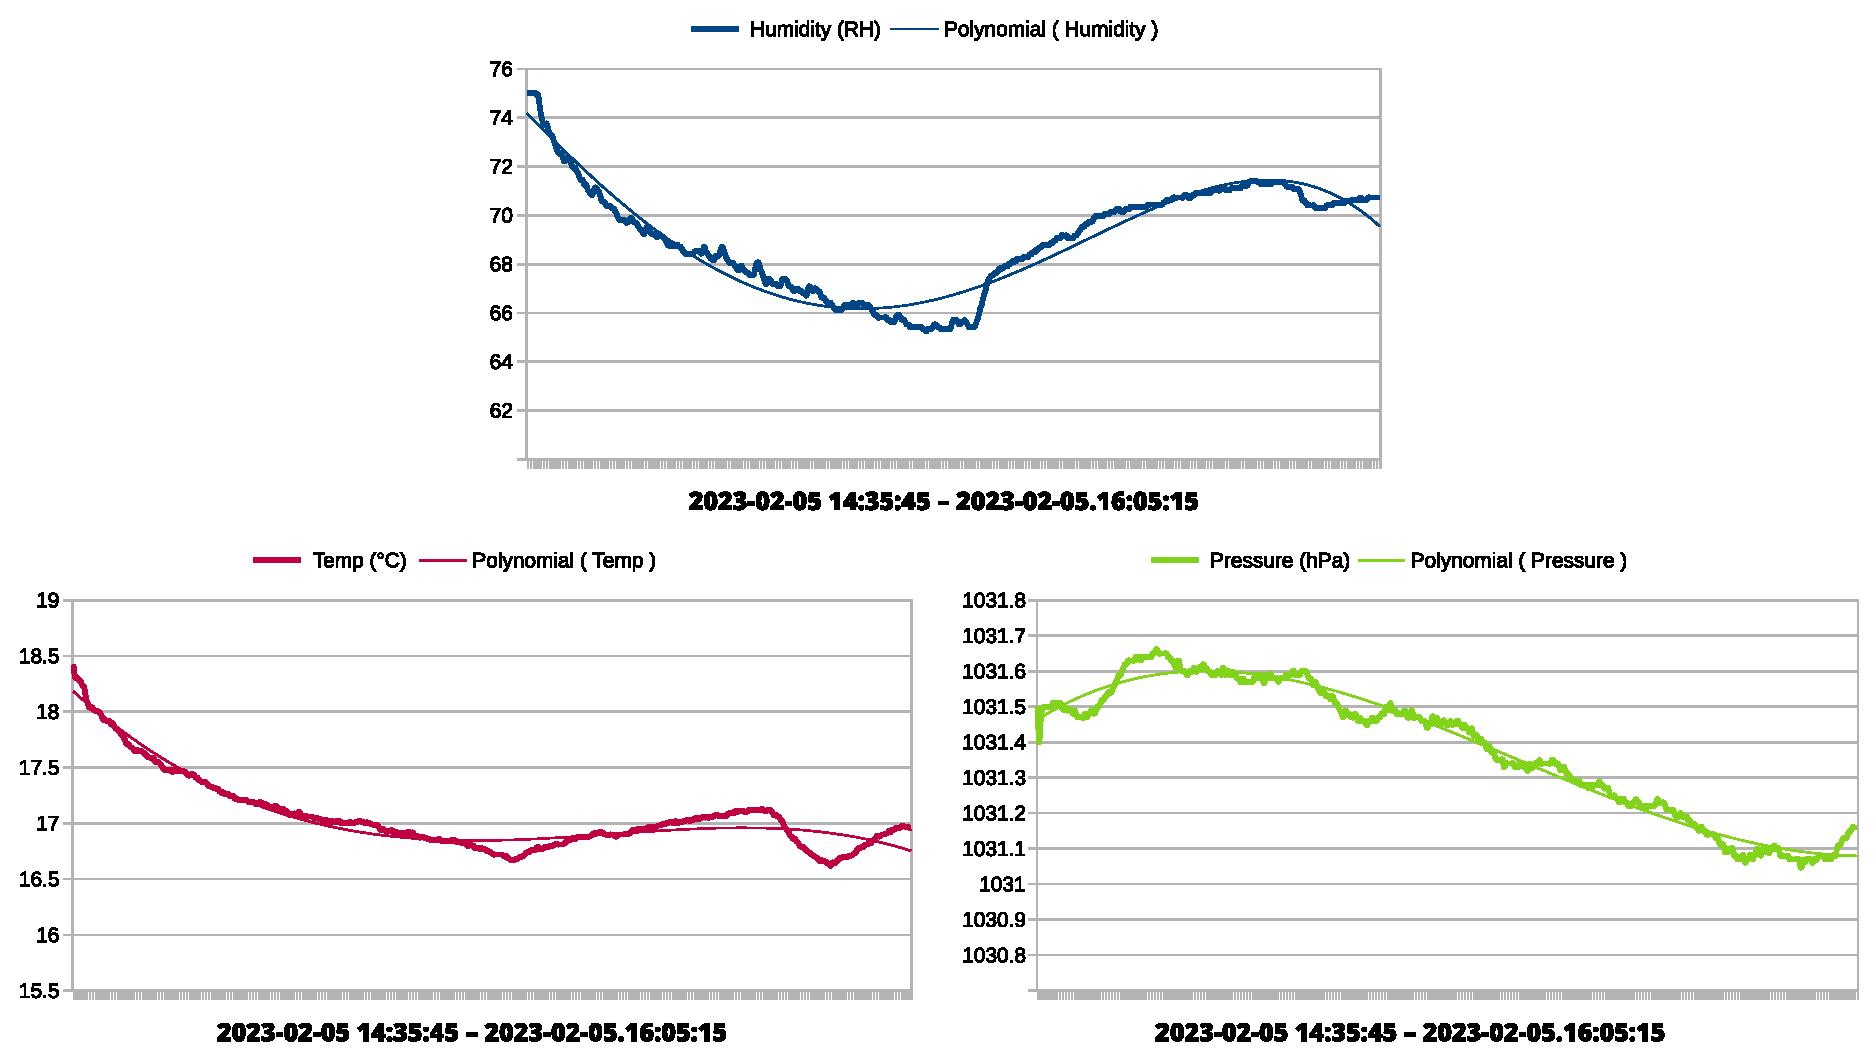
\includegraphics[width=\linewidth]{media/data.pdf}
    \end{center}


  \end{multicols*}


  \begin{multicols}{2}
    \lstinputlisting[caption={\href{https://github.com/falco-egg/sd-presentation/blob/main/weather\_station/weather\_station.ino}{weather\_station.ino}}]{./media/sketch/wetterstation.ino}
    \lstinputlisting[caption={\href{https://github.com/falco-egg/sd-presentation/blob/main/weather\_station/util.h}{util.h}}]{./media/sketch/util.h}
  \end{multicols}

  \newpage~\vfill
  \handsec{Weiterführende Literatur}
  Arduino -- \href{https://docs.arduino.cc/learn/programming/sd-guide}{Guide to Arduino \& Secure Digital (SD) Storage.}~[ENG]\\
  \hspace*{1em} {\footnotesize Artikel mit Beispielen zur Verwendung der SD Library}\\

  Arduino -- \href{hhttps://www.arduino.cc/reference/en/libraries/sd/}{SD Library}~[ENG]\\
  \hspace*{1em} {\footnotesize Dokumentation der SD Library}\\

  SD Association -- \href{https://www.sdcard.org/developers/}{SD Standard Overview}~[ENG]\\
  \hspace*{1em} {\footnotesize Weitere Informationen zu SD-Karten}\\

  David Kriesel -- \href{https://youtu.be/\_Pd5sXXMMLI}{Big Data - mal ganz anders erklärt} \& \href{https://youtu.be/0rb9CfOvojk}{BahnMining - Pünktlichkeit ist eine Zier}\\
  \hspace*{1em} {\footnotesize Beispiele interessanter Datenanalysen}\\

  Dylan Beattie -- \href{https://youtu.be/gd5uJ7Nlvvo}{Plain text}~[ENG]\\
  \hspace*{1em} {\footnotesize Ein Mahnruf zu den Feinheiten der Textkodierung und Lokalisierung in Computersystemen}\\

  \handsec{Literaturverzeichnis}
  \printbibliography[heading=none]

  Quelltext des Beispielprogramms~Wetterstation, und der \href{https://www.latex-project.org/}{\LaTeX} Dokumente (Präsentation \& Handout):\\
  \hspace*{1em} \url{https://github.com/falco-egg/sd-presentation}

  \fancyfoot[L]{\framebox[.9\linewidth][l]{\doclicenseText \hfill \doclicenseIcon}}%
\end{document}